\documentclass{article}
\usepackage[paperletter]{geometry}
\geometry{top=1.0in, bottom=1.0in, left=1.0in, right=1.0in}
\usepackage[utf8]{inputenc}
\usepackage{cancel}
\usepackage{color, colortbl}
\definecolor{Gray}{gray}{0.9}
\usepackage{tikz}
\usepackage{siunitx}
\DeclareSIUnit\atm{atm}
\usepackage{amsmath}
\usepackage{mathdots}
\usepackage{yhmath}
\usepackage{color}
\usepackage{array}
\usepackage{multirow}
\usepackage{amssymb}
\usepackage{gensymb}
\usepackage{hyperref}
\hypersetup{
colorlinks=true,
linkcolor=blue,
filecolor=magenta,      
urlcolor=blue,
citecolor=blue,
}
\urlstyle{same}
\usepackage{tabularx}
\usepackage{booktabs}
\usepackage{booktabs}
\usepackage{float}
\usepackage{multicol}
\usetikzlibrary{fadings}
\usetikzlibrary{patterns}
\usetikzlibrary{shadows.blur}
\usepackage{fancyhdr}
\pagestyle{fancy}
\lfoot[\vspace{-15pt} \hline]{\vspace{-15pt} \hline}
\rfoot[\vspace{-15pt} \hline]{\vspace{-15pt} \hline}
\cfoot[\thepage]{\thepage}
\lhead[\copyright 2020 $-$ \textit{All Rights Reserved} ]{\copyright 2020 $-$ \textit{All Rights Reserved}}
\chead[AP Physics 2]{AP Physics 2}
\rhead[Michael Brodskiy]{Michael Brodskiy}
\usepackage[symbol]{footmisc}
\renewcommand*{\thefootnote}{\fnsymbol{footnote}}
%\usepackage{everysel}
%\usepackage{ragged2e}
%\renewcommand*\familydefault{\ttdefault}
%\EverySelectfont{%
%\fontdimen2\font=0.4em% interword space
%\fontdimen3\font=0.2em% interword stretch
%\fontdimen4\font=0.1em% interword shrink
%\fontdimen7\font=0.1em% extra space
%\hyphenchar\font=`\-% to allow hyphenation
%}
\title{An Approximate Graphical and Algebraic Analysis of the Volume of an Isolated, Spherical, Sodium Laureth Sulfate and Water Solution System Placed Within a Larger System with Increasing Pressure, both Filled with the Same Ideal, Diatomic Gas and Isolated from Outside Forces}
\author{Michael \textsc{Brodskiy}}
\date{October 13, 2020}

\begin{document}

\maketitle
\begin{center}
\begin{tabular}{l r}
\underline{Date Performed}: & October 2020 \\\\ % Date the experiment was performed
\underline{Partners}: & N/A\\
\underline{Instructor}: & Mrs. Morse \\\\\\\\\\ % Instructor/supervisor
\end{tabular}
\end{center}
\newpage

\tableofcontents
\listoftables
\listoffigures
\newpage

\section{Gathered Data}

\begin{table}[H]
  \centering
  \begin{tabular}{|l|l|l|l|l|}
    \hline
    Pressure [$\si{\atm}$] & Pressure [$\si{\pascal}$] & Diameter [$\si{\meter}$] & Volume [$\si{\meter\cubed}$] & Inverse Volume [$\si{\per\meter\cubed}$] \\
    \hline
    \rowcolor{Gray} .506 & 51270.45 & .0285 & 1.21$\cdot10^{-5}$ & 82504.87 \\
    \hline
    .411 & 41644.58 & .0305 & 1.49$\cdot10^{-5}$ & 67315.44 \\
    \hline
    \rowcolor{Gray} .305 & 30904.13 & .034 & 2.06$\cdot10^{-5}$ & 48593.42 \\
    \hline
    .205 & 20771.63 & .039 & 3.11$\cdot10^{-5}$ & 32197.37 \\
    \hline
    \rowcolor{Gray} .104 & 10537.8 & .05 & 6.54$\cdot10^{-5}$ & 15279.33\\
    \hline
    \rowcolor{Gray} .057 & 5775.53 & 0 & 0 & 0\\
    \hline
  \end{tabular}
  \caption{Gathered Data}
  \label{tab:1}
\end{table}

\section{Statement of Purpose}

This laboratory experiment is intended to determine the relationship between pressure and volume in a controlled system by measuring and recording pressure and volume.

\section{Materials Used}

\begin{enumerate}

  \item Sealed container

  \item Bottle cap, dipped in soap

  \item Phone, for pressure measuring purposes

  \item Pressure pump

\end{enumerate}

\section{Procedure}

\begin{enumerate}

  \item Dip a bottle cap in soap

  \item Place bottle cap in a sealed container

  \item Change pressure (decrease in this case) in the sealed container

  \item Record the corresponding diameter and pressure values

  \item From the diameter, the volume needs to be determined using: $V=\frac{4}{3}\pi\left( \frac{d}{2} \right)^3$

  \item Finally, graphs will be produced, linearized and curved, with the vertical axis being inverse volume and volume, respectively, and the horizontal axis being pressure because it was the independent variable

    \begin{figure}[H]
      \centering
      

\tikzset{every picture/.style={line width=0.75pt}} %set default line width to 0.75pt        

\begin{tikzpicture}[x=0.75pt,y=0.75pt,yscale=-1,xscale=1]
%uncomment if require: \path (0,461); %set diagram left start at 0, and has height of 461

%Shape: Can [id:dp17510382575383798] 
\draw   (359,350.95) -- (359,360.05) .. controls (359,361.13) and (345.57,362) .. (329,362) .. controls (312.43,362) and (299,361.13) .. (299,360.05) -- (299,350.95) .. controls (299,349.87) and (312.43,349) .. (329,349) .. controls (345.57,349) and (359,349.87) .. (359,350.95) .. controls (359,352.03) and (345.57,352.9) .. (329,352.9) .. controls (312.43,352.9) and (299,352.03) .. (299,350.95) ;
%Straight Lines [id:da6852491752642553] 
\draw    (151.5,363) -- (329,362) ;
%Shape: Boxed Line [id:dp20101918104290828] 
\draw    (329,362) -- (506.5,361) ;
%Shape: Arc [id:dp936530189477714] 
\draw  [draw opacity=0] (151.5,363.16) .. controls (151.5,362.51) and (151.5,361.86) .. (151.5,361.21) .. controls (151.5,235.71) and (230.97,133.97) .. (329,133.97) .. controls (426.97,133.97) and (506.41,235.59) .. (506.5,360.99) -- (329,361.21) -- cycle ; \draw   (151.5,363.16) .. controls (151.5,362.51) and (151.5,361.86) .. (151.5,361.21) .. controls (151.5,235.71) and (230.97,133.97) .. (329,133.97) .. controls (426.97,133.97) and (506.41,235.59) .. (506.5,360.99) ;
%Curve Lines [id:da6906058744459618] 
\draw    (304.5,136) .. controls (344.5,106) and (272.5,100) .. (312.5,70) ;
%Curve Lines [id:da5971348186954979] 
\draw    (357.5,137) .. controls (397.5,107) and (325.5,101) .. (365.5,71) ;

%Curve Lines [id:da43819511514532783] 
\draw    (310.5,71) .. controls (350.5,41) and (278.5,35) .. (318.5,5) ;
%Curve Lines [id:da3524822593890953] 
\draw    (363.5,72) .. controls (403.5,42) and (331.5,36) .. (371.5,6) ;

%Shape: Arc [id:dp13203389786079556] 
\draw  [draw opacity=0] (299,350.95) .. controls (289.62,342.24) and (283.69,329.37) .. (283.69,315.01) .. controls (283.69,288.78) and (303.5,267.51) .. (327.94,267.51) .. controls (352.37,267.51) and (372.19,288.78) .. (372.19,315.01) .. controls (372.19,328.96) and (366.59,341.5) .. (357.67,350.19) -- (327.94,315.01) -- cycle ; \draw   (299,350.95) .. controls (289.62,342.24) and (283.69,329.37) .. (283.69,315.01) .. controls (283.69,288.78) and (303.5,267.51) .. (327.94,267.51) .. controls (352.37,267.51) and (372.19,288.78) .. (372.19,315.01) .. controls (372.19,328.96) and (366.59,341.5) .. (357.67,350.19) ;
%Straight Lines [id:da08347245437858009] 
\draw    (291.5,315) -- (361.5,315) ;
%Straight Lines [id:da9255606880484] 
\draw    (291.5,298.25) -- (291.5,331.75) ;
%Straight Lines [id:da9160639670883368] 
\draw    (361.5,298.25) -- (361.5,331.75) ;

% Text Node
\draw (327.94,312.01) node [anchor=south] [inner sep=0.75pt]   [align=left] {$\displaystyle d$};


\end{tikzpicture}

      \caption{Set-up of the Laboratory Experiment, $V=\frac{4}{3}\pi\left( \frac{d}{2} \right)^3$}
      \label{fig:1}
    \end{figure}

\end{enumerate}

\section{Background Knowledge}

\begin{equation}
  PV=nRT
  \label{1}
\end{equation}

\section{Graphical Analysis}

\begin{figure}[H]
  \centering
  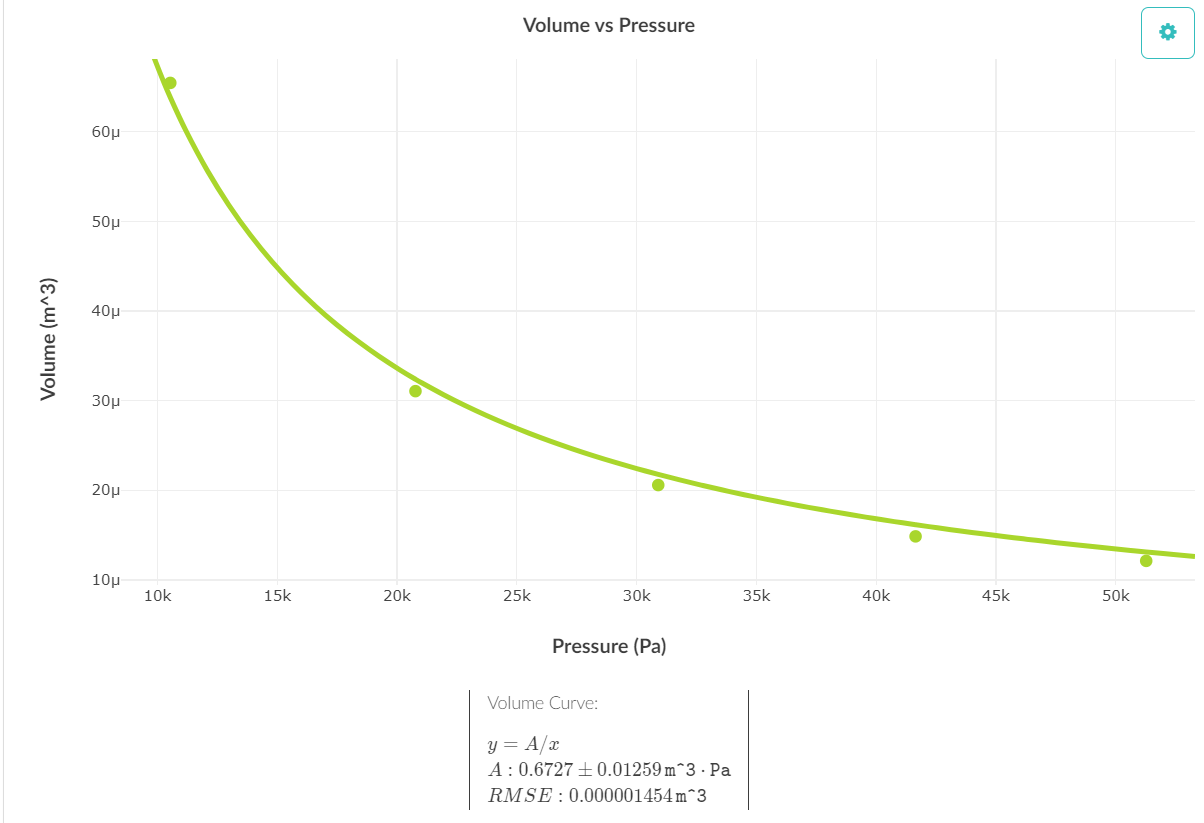
\includegraphics[width=.75\textwidth]{Figures/Curved.png}
  \caption{Curved Graph: $\frac{1}{V}=\frac{P}{nRT}$}
  \label{fig:2}
\end{figure}

\begin{figure}[H]
  \centering
  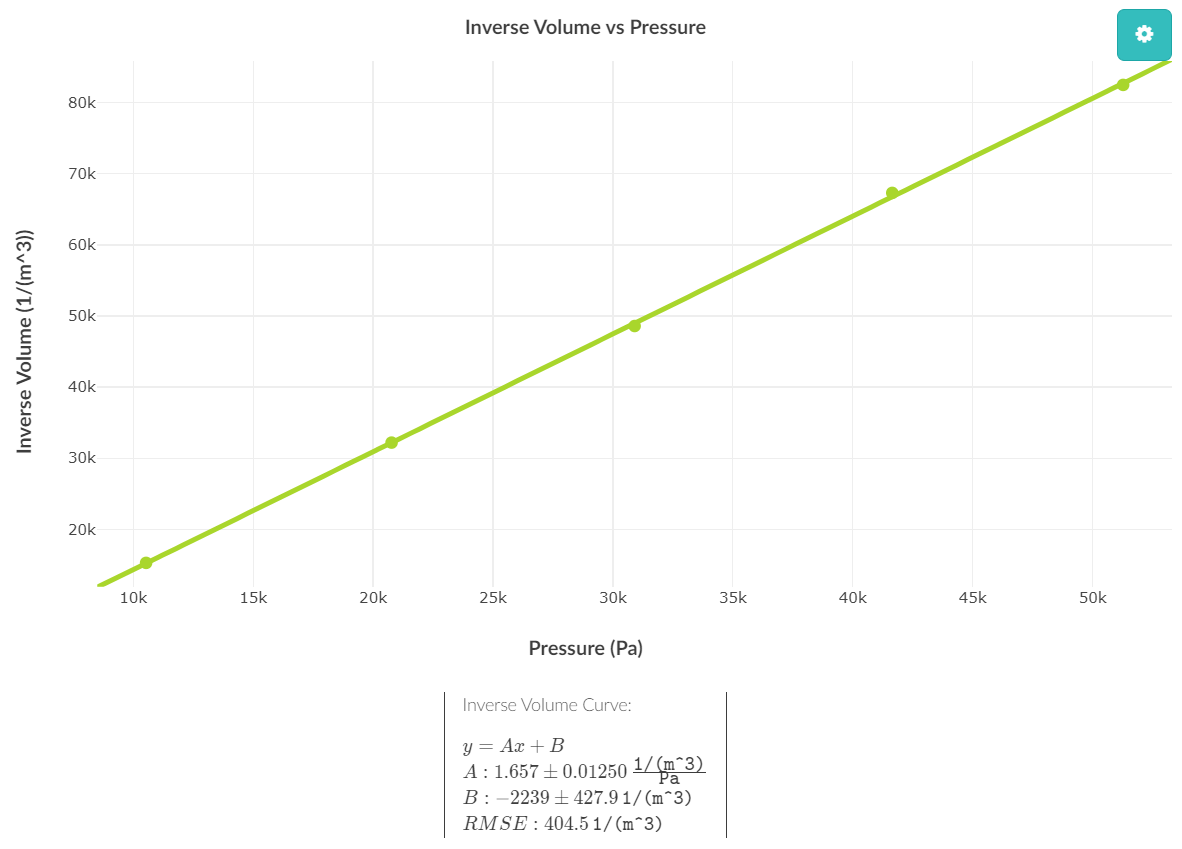
\includegraphics[width=.75\textwidth]{Figures/Linear.png}
  \caption{Linear Graph (where $I_V=V^-1$): $I_V=\frac{P}{nRT}$}
  \label{fig:3}
\end{figure}

\begin{enumerate}

  \item The curved graph is of the form $y=\frac{A}{x}$

  \item Because the graph represents an inverse correlation, the vertical column should be exponentiated to the power of negative one

\end{enumerate}

\section{Post-Lab Questions and Conclusion}

\begin{enumerate}

  \item According to the results of the experiment, there is an inverse relationship between $P$ and $V$ $\rightarrow$ $P\propto\frac{1}{V}$

  \item The slope of the line given in graph \figref{fig:3} is 1.657[$\si{\per\joule}$]

  \item The equation of the line is $I_V=\frac{P}{nRT}$, where $I_V$ represents the linearized function $\left( V^{-1} \right)^{-1}$. This means the slope may be represented as $\frac{1}{nRT}=1.657$

  \item The graph has a non-zero intercept because the volume of the bubble becomes too great and it bursts at pressure $.057[\si{\atm}]$.

  \item The vertical axis intercept shows us the theoretical volume of the bubble at 0 pressure.

  \item Following the laboratory experiment, it becomes clear that there is an inverse relationship between pressure and volume, that is, as one increases, the other decreases, which makes sense, as a gas expands, there is less pressure. A calculation of error can not be provided, as there was no actual calculation performed. One source of error is that air is not an ideal gas. This means that collisions between the particles are not perfectly elastic, and therefore, the ideal gas law \eqref{1} only serves as an approximation. One lab I think would be very interesting to see is a correlation between pressure and temperature, where the experiment is heating up and boiling water through an increase of pressure.

\end{enumerate}

\newpage
    
\end{document}
